% Standalone source for the title slide figure in slides03-data-leakage.tex.
% Compile with: pdflatex leakage_title.tex
% Then move the resulting leakage_title.pdf to ../figure/
% (Repo convention: figure_man/ = sourced assets, figure/ = generated.)
\documentclass[tikz, border=6pt]{standalone}
\usepackage{xcolor}
\usetikzlibrary{arrows.meta}

\definecolor{leakred}{HTML}{C0392B}
\definecolor{cleangreen}{HTML}{27AE60}
\definecolor{gapgray}{HTML}{555555}

\begin{document}
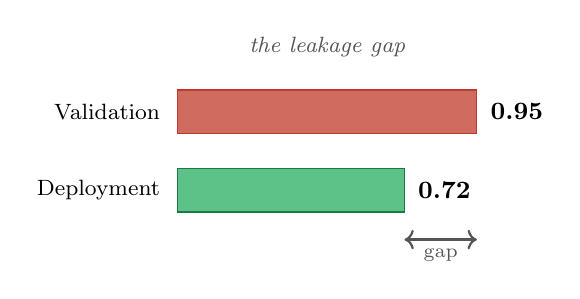
\begin{tikzpicture}[font=\small]
  % --- Validation bar (large, red -- the reported number) ---
  \fill[leakred!75]   (0, 0)    rectangle (3.80, 0.55);
  \draw[leakred]      (0, 0)    rectangle (3.80, 0.55);

  % --- Deployment bar (smaller, green -- the actual number) ---
  \fill[cleangreen!75]      (0, -1.0) rectangle (2.88, -0.45);
  \draw[cleangreen!70!black] (0, -1.0) rectangle (2.88, -0.45);

  % --- Labels on the left ---
  \node[anchor=east, font=\footnotesize] at (-0.1, 0.275)  {Validation};
  \node[anchor=east, font=\footnotesize] at (-0.1, -0.725) {Deployment};

  % --- Values on the right of the bars ---
  \node[anchor=west, font=\small\bfseries] at (3.85, 0.275)  {0.95};
  \node[anchor=west, font=\small\bfseries] at (2.93, -0.725) {0.72};

  % --- Gap annotation ---
  \draw[<->, thick, gapgray] (2.88, -1.35) -- (3.80, -1.35);
  \node[gapgray, below, font=\scriptsize] at (3.34, -1.35) {gap};

  % --- Headline ---
  \node[font=\footnotesize\itshape, anchor=south, gapgray] at (1.9, 0.85) {the leakage gap};
\end{tikzpicture}
\end{document}
